% Copyright 2018-2023 Louis Paternault
%
% This work may be distributed and/or modified under the
% conditions of the LaTeX Project Public License, either version 1.3
% of this license or (at your option) any later version.
% The latest version of this license is in
%   http://www.latex-project.org/lppl.txt
% and version 1.3 or later is part of all distributions of LaTeX
% version 2005/12/01 or later.
%
% This work has the LPPL maintenance status `maintained'.
%
% The Current Maintainer of this work is Louis Paternault

\documentclass{ltxdoc}

\usepackage{hyperref}
%\PassOptionsToPackage{draft}{pixelart} % Uncomment for quick compilation
\usepackage{graph35}
\usetikzlibrary{arrows.meta}
\usepackage[english]{babel}
\newcommand{\internationalizedempty}{\emph{Empty}}
\newcommand{\internationalizedCalculator}{Calculator}
\newcommand{\internationalizedAnchorsKeys}{Key anchors}
\newcommand{\internationalizedAnchorsReplay}{\texttt{REPLAY} key anchors}
\newcommand{\internationalizedAnchorsScreen}{Screen anchors}
\newcommand{\internationalizedAnchorsCase}{Case anchors}
\newcommand{\internationalizedKeyview}{Keywords of keys}
\usepackage{textcomp}
\usepackage{fontspec}
\usepackage{supertabular}
\usepackage{listings}
\lstset{
  language=[LaTeX]TeX,
  numbers=left,
  numberstyle=\tiny,
  backgroundcolor=\color{yellow!20},
  basicstyle=\small\color{black}\ttfamily,
  keywordstyle=\color{blue!80}\sffamily,
  commentstyle=\color{olive},
  stringstyle=\color{red},
}
\newcommand{\TikZ}{Ti\emph{k}Z}

\begin{document}

 \title{Graph35\thanks{
   This document corresponds to \textsf{graph35}~0.1.4, dated 2023-04-04.
   Home page, bug requests, etc. at \url{http://framagit.org/spalax/graph35}.
 }\\A \LaTeX{} package to display keys and screen of (some) \textsc{Casio} calculators.}
 \author{Louis Paternault\\ \texttt{spalax(at)gresille(dot)org}}

 \maketitle

 \begin{abstract}
   This package provides macros to display keys and menu items of some \textsc{Casio} calculators (including \textsc{Graph25}, \textsc{Graph35}, \textsc{Graph75} and others…).
 \end{abstract}

 \section*{Foreword}
 My dear English readers, I am really sorry… I had my French colleagues in mind when I wrote this package, so, once in a while, the main documentation is written in French. The document you are reading now is only a translation, and I fear that my English translation is worse than what you would have read if I had written it directly in English. Sorry. And good luck reading this…

 \setcounter{tocdepth}{2}
 \tableofcontents

 \section{Introduction}
 This document introduces the \textsf{graph35} package.

 \subsection{Licence}

 This work may be distributed and/or modified under the
 conditions of the \LaTeX{} Project Public License, either version 1.3
 of this license or (at your option) any later version.

 Further information can be found in the |.dtx| file used to build the |.sty| document and the main (French) documentation, available at \url{http://ctan.org/pkg/graph35}.

 \subsection{Summary}

 Section \ref{sec:install} covers installation instruction. Macros and package options are introduced in section \ref{sec:usage}. Some software developped together with this package are described in section \ref{sec:binaries}. Appendixes \ref{sec:calculators} to \ref{sec:keys} list available calculators, keys, menu items, and illustrates some options. This document does not include the implementation: it is available in the main (French) documentation.

 \section{Download and install}
 \label{sec:install}

 \subsection{\textsc{Gnu}/Linux Distribution}

 If applicable, the easiest way to get |graph35| working is by installing it by your distribution package. In Debian (and Ubuntu, and surely other distributions that inherit from Debian) it is packaged in |texlive-pictures| since version \texttt{2018.20180404-1}. So you can install it by running:

 \begin{quote}
 |sudo apt install texlive-pictures|
 \end{quote}

 \subsection{\LaTeX{} distribution}

 This package is included both in \TeX{}Live and MiK\TeX{}. It can be installed by their respective package managers.

 \subsection{Manual install}

 \begin{itemize}
 \item Download the archive:
 \begin{description}
 \item[Stable version] \url{http://mirrors.ctan.org/graphics/graph35.zip}
 \item[Development version] \url{https://framagit.org/spalax/graph35/repository/archive.zip?ref=main}
 \end{description}
 \item Uncompress the archive.
 \item Compile the package : |latex graph35.ins|
 \item Move the several |.sty| files in a directory that is part of the \LaTeX{} path.
 \end{itemize}

 \section{Usage}
 \label{sec:usage}

 \subsection{Supported calculators}

 \begin{description}
   \item[Case and keys] The macros can display case and keys of the \textsc{Graph35} calculator only (although it can have another name in another country).
 \item[Screen] This package implements screen items of models \textsc{Graph25}, \textsc{Graph35}, \textsc{Graph75}, \textsc{fx-9860gii}, \textsc{fx-9750gii}, and others.
 \end{description}

 \subsection{Package options}

 This package has a single |color| option, which is set to |color=real| by default.

 This option accepts two values: |real| and |blackandwhite|, defining the default key and case color. See next section for more details.

 Moreover, this is not, strictly speaking, a package option, but it is possible, to make compilation faster, to add the following line before loading this package.

 \changes{v0.1.2}{2022/11/19}{Changed package used to draw menus.}
 \begin{lstlisting}
 \PassOptionsToPackage{draft}{pixelart0}
 \end{lstlisting}

 This line will disable pixelart images (mainly the |\function| macros, see part \ref{sec:function}). Indeed, having a lot of those macros can make compilation very long, and adding this line can make it faster\footnote{For instance, on my computer, adding this line to this files make compiling thirty times faster, from eight minutes to sixteen seconds.}.

 \subsection{Colors}
 \label{sec:colors}

 \subsubsection{Preset colors}

 You can chose the case and key colors from preset profiles, or customize them. Those preset profiles are:
 \begin{description}
 \item[real] \key[shift, alpha, color=real]{ACON} Realistic colors, but can be hard to read when printed in black and white.
 \item[blackandwhite] \key[shift, alpha, color=blackandwhite]{ACON} Black and white, hight contrast, that will be easier to read when printed.
 \end{description}

 \subsubsection{Color choice}

 There are several ways to set colors.

 \begin{itemize}
   \item Package argument |color| defines the default color to use (which can be later overloaded using option |color| of the macros). For instance, to make all drawing black and white, load the package using the following line.

     \begin{lstlisting}
     \usepackage[color=blackandwhite]{graph35}
     \end{lstlisting}

     By default, realistic color are used (|color=real|).
   \item Option |color| of macros |\key| and |\calculator| can have an additional value |default|. Using this explicitely uses the default color defined while loading the package.
 \item
 \DescribeMacro{\setgraphcolor}
 At last, default color can be redefined at any time using macro |\setgraphcolor|\marg{color}. For instance, if the package was loaded with option |color=blackandwhite|, use \lstinline|\setgraphcolor{real}| to use the |real| colors by default.
 \end{itemize}

 \subsubsection{Custom colors}

 Arbitrary colors can also be used, by defining the following colors.

 \begin{description}
   \item |graph35ACON| : Key |ACON| \key{ACON}.
   \item |graph35ACONBORDER| : Border of key |ACON|.
   \item |graph35ALPHA| : Key |ALPHA| \key{ALPHA}.
   \item |graph35ALPHABORDER| : Border of key |ALPHA|.
   \item |graph35SHIFT| : Key |SHIFT| \key{SHIFT}.
   \item |graph35SHIFTBORDER| : Border of key |SHIFT|.
   \item |graph35SCREEN| : Screen pixels.
   \item |graph35SCREENBG| : Screen background.
   \item |graph35CASE| : Case.
   \item |graph35CASEBORDER| : Case border.
   \item |graph35EXE| : Key |EXE| \key{EXE}.
   \item |graph35EXEBORDER| : Border of key |EXE|.
   \item |graph35NUMBER| : Number keys.
   \item |graph35NUMBERBORDER| : Border of number keys.
   \item |graph35KEYTEXT| : Text on keys.
   \item |graph35ALPHATEXT| : Text \emph{alpha} above keys.
   \item |graph35SHIFTTEXT| : Text \emph{shift} above keys.
 \end{description}

 \colorlet{graph35KEYTEXT}{green}
 \colorlet{graph35SHIFTTEXT}{orange}
 \definecolor{graph35ALPHATEXT}{RGB}{0, 0, 255}
 \definecolor{graph35NUMBER}{RGB}{200, 200, 200}
 \colorlet{graph35NUMBERBORDER}{graph35NUMBER}

 Those colors are color names as defined by package |xcolor|, and can be defined using macros from this package. For instance, to display \key[shift, alpha]{7}, use the following code:

 \begin{lstlisting}
 \colorlet{graph35KEYTEXT}{green}
 \colorlet{graph35SHIFTTEXT}{orange}
 \definecolor{graph35ALPHATEXT}{RGB}{0, 0, 255}
 \definecolor{graph35NUMBER}{RGB}{200, 200, 200}
 \colorlet{graph35NUMBERBORDER}{graph35NUMBER}
 
 \key[shift, alpha]{7}
 \end{lstlisting}

 \setgraphcolor{real}

 \subsection{Calculators}

 \DescribeMacro{\calculator}
 Right now, only one model is available: \textsc{graph35+}.

 Syntax is: \lstinline|\calculator|\oarg{color, scale}\marg{model}.

 \begin{itemize}
 \item \marg{model} The list of available models is available in appendix \ref{sec:calculators} (page \pageref{sec:calculators}).
 \item \oarg{color} Change calculator colors (see previous part \ref{sec:colors}).
 \item \oarg{scale} Change calculator scale. The drawing you get might not be what you expect: see part \ref{sec:scale} for more information.
 \end{itemize}

 For instance, command \lstinline|\calculator[color=real]{graph35+E}| displays a calculator ten times bigger than the following calculator (scaled down here for readability; a bigger version is displayed in appendix \ref{sec:calculators}, page \pageref{sec:calculators}).

 \begin{center}
 \scalebox{.1}{%
   \calculator{graph35+E}
 }
 \end{center}

 \DescribeMacro{\tikzcalculator}
 One can include a calculator in a \TikZ{} drawing, using command \lstinline|\tikzcalculator|\marg{model}. This command takes a single argument \marg{model}, and displays a calculator around coordinates $(0; 0)$. To draw a calculator elsewhere, or with another scale, use the |scope| environment, as in the following example.

 \begin{lstlisting}
 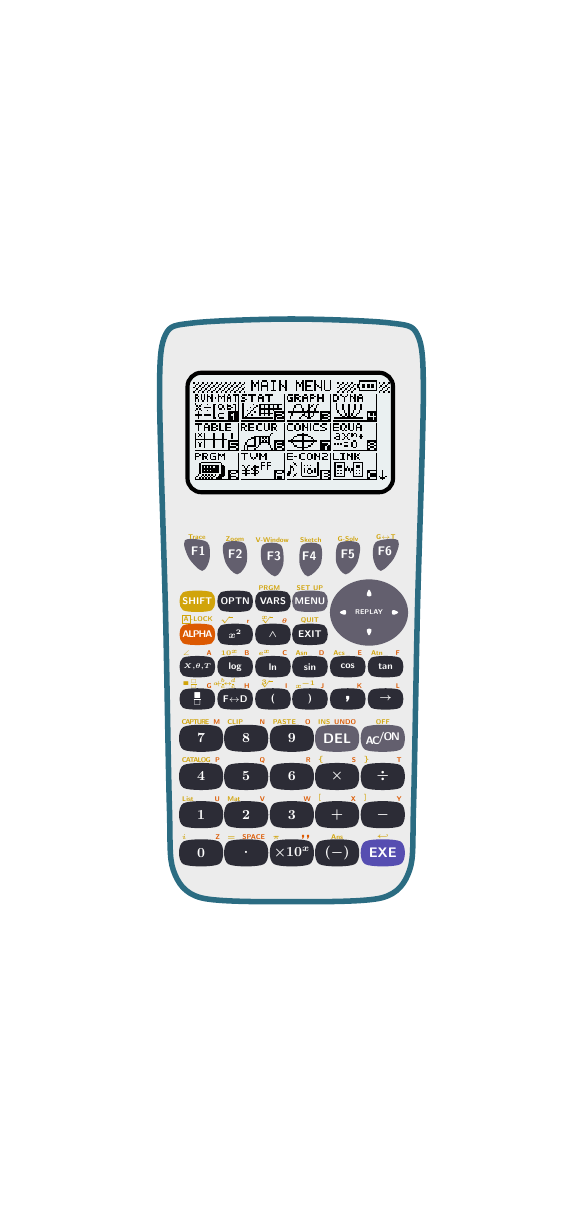
\begin{tikzpicture}
   \begin{scope}[shift={(1, 2)}, scale=.5]
     \tikzcalculator{graph35+E}
   \end{scope}
 \end{tikzpicture}
 \end{lstlisting}

 Anchors are defined for each keys, case borders, and screen, to be used within your \TikZ figures. See appendix \ref{sec:anchors} for more information.

 \subsection{Keys}

 \DescribeMacro{\key}
 \changes{v0.1.4}{2023/04/04}{Changed design of the $X\theta{}T$ key.}
 To draw a calculator key, use:
 \begin{center}
 \lstinline|\key|\oarg{color, prefix, suffix, scale, shift, alpha}\marg{key}.
 \end{center}

 For instance, \lstinline|\key[color=blackandwhite]{DEL}| displays \key[color=blackandwhite]{DEL} while \lstinline|\key[shift, alpha]{DEL}| displays \key[shift, alpha]{DEL}.

 Arguments are:
 \begin{itemize}
 \item \marg{key} Key name to display (for instance \lstinline|1| for \key{1}, and \lstinline|EXE| for \key{EXE}). Key name is more or less what is displayed on it. Key names are available as a list in appendix \ref{sec:keylist}, or as a calculator with captions in figure \ref{fig:keyview}.
 \item \oarg{color, scale} Scale and color of key. Those options have the same syntax and limitations as options of command \lstinline|calculator| (see section \ref{sec:colors} for colors, and \ref{sec:scale} for scale).
 \item \oarg{shift, alpha} Those options enable or disable yellow and red text describing the key meaning when pressed after the \key{SHIFT} or \key{ALPHA} keys. By default, those texts are hidden (equivalent to \texttt{shift=false, alpha=false}) ; to enable the, use \texttt{shift=true} and \texttt{alpha=true} or \texttt{shift} and \texttt{alpha}.
 \item \oarg{prefix, suffix} For each key, anchors are defined, allowing references to the key in \TikZ{} pictures (for instance, they are used to draw figure \ref{fig:keyview}, page \pageref{fig:keyview}). By default, anchor names are \texttt{key} followed by the key name (for instance \texttt{keyDEL} for the \texttt{DEL} key). The |prefix| and |suffix| options make the anchor names customizable (as used in the following pictures). With those options, two keys can have different anchors on the same figure, making it possible to use each of those keys.
   Those options also define anchor names for \texttt{SHIFT} et \texttt{ALPHA} texts.
 \begin{center}
 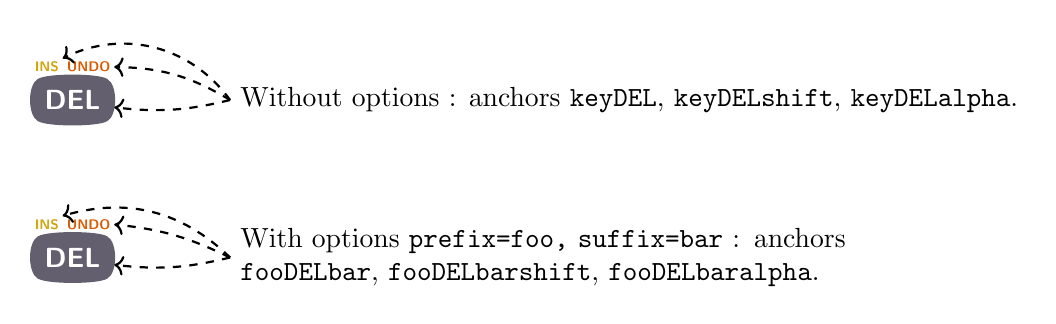
\begin{tikzpicture}[thick]
 \tikzkey[shift, alpha]{DEL}{(0, 2)}
 \tikzkey[shift, alpha, prefix=foo, suffix=bar]{DEL}{(0, 0)}

 \draw (2, 2) node[anchor=west]{Without options : anchors \texttt{keyDEL}, \texttt{keyDELshift}, \texttt{keyDELalpha}.};
 \draw (2, 0) node[anchor=west, text width={8cm}]{With options \texttt{prefix=foo, suffix=bar} : anchors \texttt{fooDELbar}, \texttt{fooDELbarshift}, \texttt{fooDELbaralpha}.};

 \draw[dashed] (2, 2) edge[->, bend left=10] (keyDEL);
 \draw[dashed] (2, 2) edge[->, bend right=40] (keyDELshift.north east);
 \draw[dashed] (2, 2) edge[->, bend right=15] (keyDELalpha.east);
 \draw[dashed] (2, 0) edge[->, bend left=10] (fooDELbar);
 \draw[dashed] (2, 0) edge[->, bend right=30] (fooDELbarshift.north east);
 \draw[dashed] (2, 0) edge[->, bend right=10] (fooDELbaralpha.east);
 \end{tikzpicture}
 \end{center}
 The anchor names are listed in appendixes \ref{sec:anchorskey} and \ref{sec:anchorsreplay}.
 \item Peeking at the source code, you may see that more options are used. Those options are not described here because they are not meant to be used by final users, and might change in a later version without notice.
 \end{itemize}

 \DescribeMacro{\tikzkey}
 As with |\calculator| and |\tikzcalculator|, macro |\tikzkey| does the same as |\key|, excepted that it is meant to be called from within a \TikZ{} environment. Its syntax is:
 \begin{center}
 |\tikzkey|\oarg{options}\marg{key}\marg{coordinates}
 \end{center}

 Its arguments are
 \begin{itemize}
 \item \oarg{options}: same options as macro |\key| ;
 \item \marg{key}: name of the key ;
 \item \marg{coordinates}: coordinates the key is drawn around.
 \end{itemize}

 \subsection{Screen}

 Three macros can be used to draw parts of the screen: menu items, captions of function keys, battery level.

 \subsubsection{Menu}

 \DescribeMacro{\menu}
 Macro |\menu|\marg{icon}\marg{shortcut} draws an icon from the main menu. For instance, |\menu{RUNMAT}{A}| displays \menu{RUNMAT}{A}. Shortcut (the character at the bottom right corner of the item) is independant from the icon, because depending of the calculator model or its version, it can change.

 Appendix \ref{sec:menu} is a list of every menu icon and shortcut.

 \DescribeMacro{\tikzmenu}
 The |\tikzmenu| macro draws a menu item in a \TikZ{} environment. Its syntax is:
 \begin{center}
 |\tikzmenu|\oarg{options}\marg{icon}\marg{shortcut}\marg{coordinates}
 \end{center}
 
 Its arguments are:

 \begin{itemize}
 \item \marg{icon} and \marg{shortcut}: same meaning as the corresponding |\menu| options;
 \item \marg{coordinates}: coordinates of the top-left corner of the menu item;
 \item \oarg{options}: some options, that are passed as-is to the |\bwpixelart| macro (from the |pixelart0| package). They can be used to change the scale and color of the drawing (for instance |scale=.5, color=red|).
 \end{itemize}

 \subsubsection{Functions}

 \DescribeMacro{\function}
 The |\function|\marg{function} macro displays the caption of the keys \key{F1} to \key{F6} (for instance \function{aplusbx} or \function{question-b}). Available pixel-arts are listed in appendix \ref{sec:function}.

 \DescribeMacro{\tikzfunction}
 Macro |\tikzfunction|\oarg{options}\marg{function}\marg{coordinates} is the same as |\function|, but from within a \TikZ{} environment. The \marg{function} argument is the same as for macro |\function|; see macro |\tikzmenu| for the meaning of arguments \oarg{options} and \marg{coordinates}.

 \subsubsection{Battery}

 \DescribeMacro{\battery}
 Macro |\battery|\marg{state} displays the state of charge of the battery (for instance  \battery{medium}). Available pixel-arts (and arguments) are listed in appendix \ref{sec:battery}.

 \DescribeMacro{\tikzbattery}
 Macro |\tikzbattery|\oarg{options}\marg{state}\marg{coordinates} is identical to macro |\battery|, but from within a \TikZ{} environment. Its \marg{state} argument is the same as for |\battery|; see macro |\tikzmenu| for the meaning of arguments \oarg{options} and \marg{coordinates}.

 \subsection{Scaling}
 \label{sec:scale}

 Option |scale| used to set size of calculators and keys does not change line width or border radius. The unexpected result is the following drawing of a calculator at a $^1/_{10}$ scale: the case border (green) is too big, and the screen is almost an ellipsis (among other flaws).

 \begin{center}
 \calculator[scale=.1]{graph35+E}.
 \end{center}

 There are several solutions to fix this, but none of them is perfect, which is why they are not implemented.

 \begin{itemize}
   \item Get used to those flaws. Indeed, for small scale changes, they are barely noticable.
   \item Embed the drawing in a |\scalebox| or |\resizebox| macro: command |\resizebox{.1}{\calculator{graph35+E}}| gives the following drawing.
     \begin{center}
       \scalebox{.1}{\calculator{graph35+E}}
     \end{center}
   \item Use option |transform canvas| from the |pgf| package (for instance: |\begin{tikzpicture}[scale=.1, transform canvas={scale=.1}]…|. Line width and border radius will be correctly scaled, but the bounding box will not be changed, neither will be the coordinates (thus anchors will be useless).
   \end{itemize}

 At last, when including drawings in a |tikzpicture| environment using the |scale| option, do not forget to add option |tranrsform shape|, so that bounding box is also changed.

 \section{Binaries}
 \label{sec:binaries}

 A few Python3 software are maintained together with this \LaTeX{} package. They are not distributed with it, so they have to be downloaded directly from the code repository. They are specialized enough to share this package repository, but if you were to use them for something else, good for you!

 Most of those handle |.pxl| files. This is a custom file format, coding a pixel-art picture as lines of |0|s and |1|s. Each menu, battery, function icon is stored as one of those files, and converted to \LaTeX{} code before being included in this package.

 \begin{itemize}
 \item[|catpxl|] Display a |.pxl| file to the terminal.
 \item[|completefunctionchars|] Each function icon has its readable characters associated to it (it is used in appendix \ref{sec:function}). This software look for function icons without such characters, and asks user for them.
 \item[|generate.keys| and |generate.pixelart|] Generate the \LaTeX{} files generating the pixel-art and keys, from the source files in this repository.
 \item[|screenshot2pixelart|] Parse a calculator screenshot to find new function and menu icons.
 \end{itemize}

 \appendix

 \section{Calculators}
 \label{sec:calculators}

 Here is the list of available calculators, together with their keyword (used as argument for macros |\calculator| and |\tikzcalculator|).

 \input{doc/calculators.tex}

 \section{Anchors}
 \label{sec:anchors}

 Anchors of keys, shift and alpha texts, screen, etc.

 \subsection{Anchors of keys}
 \label{sec:anchorskey}

 Each key defines the anchors shown in figure \ref{fig:anchors:key}.
 \input{doc/anchors-key.tex}

 \subsection{Anchors of key \texttt{REPLAY}}
 \label{sec:anchorsreplay}

 The |REPLAY| key defines some additionnal anchors, for each of its arrows. They are illustrated in figure \ref{fig:anchors:replay}.

 \input{doc/anchors-replay.tex}

 \subsection{Screen anchors}

 Anchors of the screen are illustrated in figure \ref{fig:anchors:screen}.

 \input{doc/anchors-screen.tex}

 \subsection{Case anchors}

 Anchors of the case are illustrated in figure \ref{fig:anchors:case}.

 \input{doc/anchors-case.tex}

 \section{Pixel art}
 \label{sec:pixelart}

 \subsection{Menu}
 \label{sec:menu}

 Two special icons and shortcuts are available: |black|, which produces a black pixel-art; and |blank|, which produces nothing.

 \subsubsection{Icons}

 \begin{multicols}{2}
 \input{doc/pixelart-menu.tex}
 \end{multicols}

 \subsubsection{Shortcuts}

 \begin{multicols}{2}
 \input{doc/pixelart-menuchar.tex}
 \end{multicols}

 \subsection{Functions}
 \label{sec:function}

 Available pixel arts are sorted according to the visible characters (latin letters and figures). To find the keyword corresponding to the picture you want, look at its visible characters, and find your picture in the corresponding part of this index.

 For example, no character is visible on \function{battery} or \function{GREEK} (indeed, letters of \function{GREEK} are greek letters, not latin ones); on \function{Sacn-b}, letters |acn| are visible; on \function{tcomplexpolar-b}, only the letter |r| is visible; and so on.

 \begin{multicols}{3}
 \input{doc/pixelart-function.tex}
 \end{multicols}

 \subsection{Battery}
 \label{sec:battery}

 List of status of battery charge.

 \begin{multicols}{3}
 \input{doc/pixelart-battery.tex}
 \end{multicols}

 \section{Keys}
 \label{sec:keys}

 \subsection{List of keys}

 Sorting order is arbitrary. To find them on a calculator, see figure \ref{fig:keyview}.

 \input{doc/key-view.tex}

 \label{sec:keylist}
 \begin{multicols}{3}
 \input{doc/key-list.tex}
 \end{multicols}

 \addcontentsline{toc}{section}{List of figures}
 \listoffigures

\end{document}
